\documentclass{article}
\usepackage[margin=1.5cm]{geometry}
\usepackage[parfill]{parskip}
\usepackage[utf8]{inputenc}
\usepackage{amsmath,amssymb,amsfonts,amsthm}
\usepackage{algorithm, algpseudocode, algcompatible}
\usepackage{graphicx, hyperref}

\author{Zaccarie Kanit}
\date{22/07/2025}

\title{Prime arithmetic}

\usepackage{filecontents}

\begin{filecontents}{lecture-tum-aci-ss2025-U4.bib}
@book{HAC,
  added-at = {2007-04-16T14:16:26.000+0200},
  author = {Menezes, Alfred J. and van Oorschot, Paul C. and Vanstone, Scott A.},
  biburl = {https://www.bibsonomy.org/bibtex/21fb86a3afb62bbb4bc2f94a0299a4d59/kidloc},
  interhash = {d5837a554ce2ffd49f551045400e244c},
  intrahash = {1fb86a3afb62bbb4bc2f94a0299a4d59},
  keywords = {cryptography handbook programming reference security},
  publisher = {CRC Press},
  timestamp = {2007-04-16T14:16:26.000+0200},
  title = {Handbook of Applied Cryptography},
  url = {http://www.cacr.math.uwaterloo.ca/hac/},
  year = 2001
}
\end{filecontents}

\usepackage{biblatex}
\addbibresource{lecture-tum-aci-ss2025-U4.bib}
\nocite{*}

\begin{document}
\maketitle

\section*{Exercise \#1}

1. Write the operand scanning multiplication algorithm (Alg. 12) for $m=n=3$.

2. Provide a graphical representation of the operand scanning multiplication algorithm  (Alg. 12) for $m=n=3$: represent the sequence how the partial products
$a_ib_j$ are computed and added together including the carries (Line 6, Alg. 12).

\subsection*{Response}

\begin{enumerate}
    \item \textbf{Algorithm Overview}

The operand scanning multiplication algorithm computes the product of two multi-precision integers represented in radix-$2^w$ form. For $m = n = 3$, we multiply two 3-digit numbers to produce a 6-digit result.

\subsubsection*{Input and Output}
\begin{itemize}
    \item \textbf{Input:} $A = (a_0, a_1, a_2)$ and $B = (b_0, b_1, b_2)$ where each digit is in base $2^w$
    \item \textbf{Output:} $P = (p_0, p_1, p_2, p_3, p_4, p_5)$ such that $P = A \times B$
\end{itemize}

\subsubsection*{Step-by-Step Algorithm Execution}
\begin{itemize}
  \item \textbf{Initialization}
  Set all product digits to zero:
  \begin{align*}
  (p_0, p_1, p_2, p_3, p_4, p_5) \leftarrow (0, 0, 0, 0, 0, 0)
  \end{align*}
\end{itemize}

\subsubsection*{Main Computation Loop}

The algorithm processes each digit $a_i$ of the first operand sequentially.
\begin{itemize}

\item \textbf{Iteration $i = 0$ (Processing $a_0$)}
Initialize carry: $u \leftarrow 0$

$\rightarrow$ \textbf{Inner loop for $j = 0, 1, 2$:}
\begin{align*}
j = 0: \quad & z \leftarrow a_0 b_0 + p_0 + u = a_0 b_0 + 0 + 0 = a_0 b_0 \\
& v \leftarrow z \bmod 2^w, \quad u \leftarrow \lfloor z/2^w \rfloor \\
& p_0 \leftarrow v \\[0.5em]
j = 1: \quad & z \leftarrow a_0 b_1 + p_1 + u = a_0 b_1 + 0 + u \\
& v \leftarrow z \bmod 2^w, \quad u \leftarrow \lfloor z/2^w \rfloor \\
& p_1 \leftarrow v \\[0.5em]
j = 2: \quad & z \leftarrow a_0 b_2 + p_2 + u = a_0 b_2 + 0 + u \\
& v \leftarrow z \bmod 2^w, \quad u \leftarrow \lfloor z/2^w \rfloor \\
& p_2 \leftarrow v
\end{align*}

Set final carry: $p_3 \leftarrow u$

\item \textbf{Iteration $i = 1$ (Processing $a_1$)}
Initialize carry: $u \leftarrow 0$

$\rightarrow$ \textbf{Inner loop for $j = 0, 1, 2$:}
\begin{align*}
j = 0: \quad & z \leftarrow a_1 b_0 + p_1 + u = a_1 b_0 + p_1 + 0 \\
& v \leftarrow z \bmod 2^w, \quad u \leftarrow \lfloor z/2^w \rfloor \\
& p_1 \leftarrow v \\[0.5em]
j = 1: \quad & z \leftarrow a_1 b_1 + p_2 + u \\
& v \leftarrow z \bmod 2^w, \quad u \leftarrow \lfloor z/2^w \rfloor \\
& p_2 \leftarrow v \\[0.5em]
j = 2: \quad & z \leftarrow a_1 b_2 + p_3 + u \\
& v \leftarrow z \bmod 2^w, \quad u \leftarrow \lfloor z/2^w \rfloor \\
& p_3 \leftarrow v
\end{align*}

Set final carry: $p_4 \leftarrow u$

\item \textbf{Iteration $i = 2$ (Processing $a_2$)}
Initialize carry: $u \leftarrow 0$

$\rightarrow$ \textbf{Inner loop for $j = 0, 1, 2$:}
\begin{align*}
j = 0: \quad & z \leftarrow a_2 b_0 + p_2 + u = a_2 b_0 + p_2 + 0 \\
& v \leftarrow z \bmod 2^w, \quad u \leftarrow \lfloor z/2^w \rfloor \\
& p_2 \leftarrow v \\[0.5em]
j = 1: \quad & z \leftarrow a_2 b_1 + p_3 + u \\
& v \leftarrow z \bmod 2^w, \quad u \leftarrow \lfloor z/2^w \rfloor \\
& p_3 \leftarrow v \\[0.5em]
j = 2: \quad & z \leftarrow a_2 b_2 + p_4 + u \\
& v \leftarrow z \bmod 2^w, \quad u \leftarrow \lfloor z/2^w \rfloor \\
& p_4 \leftarrow v
\end{align*}

Set final carry: $p_5 \leftarrow u$

\end{itemize}


\subsubsection*{Algorithm Summary}

\begin{algorithm*}
\caption{Operand Scanning Multiplication for $m = n = 3$}
\begin{algorithmic}[1]
\REQUIRE $A = (a_0, a_1, a_2)$, $B = (b_0, b_1, b_2)$
\ENSURE $P = (p_0, p_1, p_2, p_3, p_4, p_5)$ such that $P = A \times B$
\STATE $(p_0, p_1, p_2, p_3, p_4, p_5) \leftarrow (0, 0, 0, 0, 0, 0)$
\FOR{$i = 0$ to $2$}
    \STATE $u \leftarrow 0$
    \FOR{$j = 0$ to $2$}
        \STATE $z \leftarrow a_i b_j + p_{i+j} + u$
        \STATE $v \leftarrow z \bmod 2^w$
        \STATE $u \leftarrow \lfloor z/2^w \rfloor$
        \STATE $p_{i+j} \leftarrow v$
    \ENDFOR
    \STATE $p_{3+i} \leftarrow u$
\ENDFOR
\end{algorithmic}
\end{algorithm*}

\subsubsection*{Key Properties}

\begin{itemize}
    \item \textbf{Time Complexity:} $O(mn) = O(9)$ operations for $m = n = 3$
    \item \textbf{Space Complexity:} $O(m+n) = O(6)$ for storing the result
    \item \textbf{Carry Propagation:} Each inner loop handles carries from digit multiplication
    \item \textbf{Index Pattern:} Product digit $p_{i+j}$ accumulates contributions from $a_i \times b_j$
\end{itemize}

\subsubsection*{Visualization of Computation Pattern}

The algorithm computes partial products in the following pattern:
\begin{align*}
\begin{array}{c|ccc}
    & b_0 & b_1 & b_2 \\
\hline
a_0 & p_0 & p_1 & p_2 \\
a_1 & p_1 & p_2 & p_3 \\
a_2 & p_2 & p_3 & p_4 \\
\end{array}
\end{align*}

Each cell $(i,j)$ contributes $a_i \times b_j$ to position $p_{i+j}$, with carries propagated to higher positions.

\item I think that this operation is similar to the carry save multiplier in hardware implementation, 
that is why I just include a generic graphic of this element.

\begin{figure}[hbt]
    \centering
    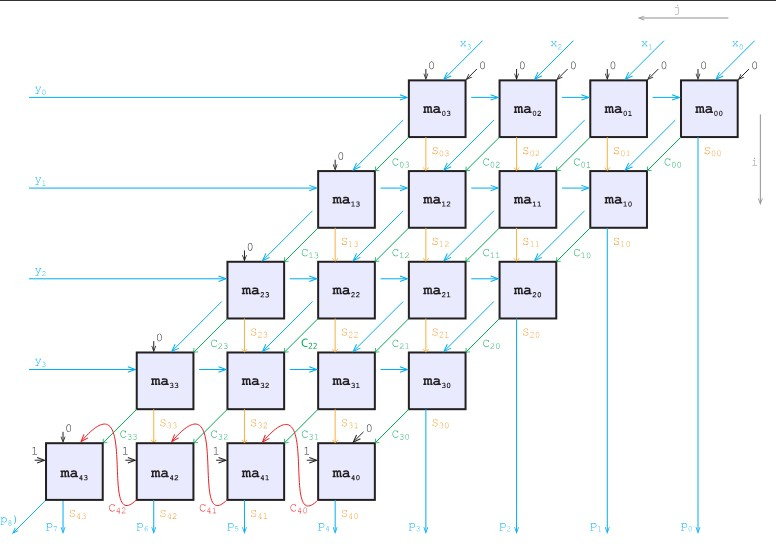
\includegraphics[width=0.5\textwidth]{carry_save_mult.jpeg}
    \caption{Graph of a carry save multiplier}
    % \caption{\href{https://coertvonk.com/wp-content/logic-simulation/multiplier/4-bit%20carry-save.svg}{Graph of a carry save multiplier}}
    \label{fig:carry_save_mult}
\end{figure}
  
\end{enumerate}

\section*{Exercise \#2}

1. Write the operand scanning multiplication algorithm (Alg. 12) for $m=n=3$ and $A=B$.

2. Optimize the operand scanning multiplication algorithm (Alg. 12) when $A=B$: write the optimized algorithm.

3. Provide a graphical representation of the optimized operand scanning multiplication algorithm  (Alg. 12) when $A=B$ and $m=n=3$.

\subsection*{Response}

\section{Part 1: Operand Scanning Multiplication for $A = B$ (m = n = 3)}

When $A = B$, we are computing $A^2$ using the standard multiplication algorithm.

\subsection{Input and Output}
\begin{itemize}
    \item \textbf{Input:} $A = (a_0, a_1, a_2)$ where each digit is in base $2^w$
    \item \textbf{Output:} $P = (p_0, p_1, p_2, p_3, p_4, p_5)$ such that $P = A^2$
\end{itemize}

\subsection{Step-by-Step Algorithm Execution for $A = B$}

\subsubsection*{Initialization}
\begin{align*}
(p_0, p_1, p_2, p_3, p_4, p_5) \leftarrow (0, 0, 0, 0, 0, 0)
\end{align*}

\subsubsection*{Iteration $i = 0$ (Processing $a_0$)}
Initialize carry: $u \leftarrow 0$
\begin{align*}
j = 0: \quad & z \leftarrow a_0 \cdot a_0 + p_0 + u = a_0^2 \\
& v \leftarrow z \bmod 2^w, \quad u \leftarrow \lfloor z/2^w \rfloor, \quad p_0 \leftarrow v \\[0.5em]
j = 1: \quad & z \leftarrow a_0 \cdot a_1 + p_1 + u \\
& v \leftarrow z \bmod 2^w, \quad u \leftarrow \lfloor z/2^w \rfloor, \quad p_1 \leftarrow v \\[0.5em]
j = 2: \quad & z \leftarrow a_0 \cdot a_2 + p_2 + u \\
& v \leftarrow z \bmod 2^w, \quad u \leftarrow \lfloor z/2^w \rfloor, \quad p_2 \leftarrow v
\end{align*}
Set final carry: $p_3 \leftarrow u$

\subsubsection{Iteration $i = 1$ (Processing $a_1$)}
Initialize carry: $u \leftarrow 0$
\begin{align*}
j = 0: \quad & z \leftarrow a_1 \cdot a_0 + p_1 + u \\
& v \leftarrow z \bmod 2^w, \quad u \leftarrow \lfloor z/2^w \rfloor, \quad p_1 \leftarrow v \\[0.5em]
j = 1: \quad & z \leftarrow a_1 \cdot a_1 + p_2 + u = a_1^2 + p_2 + u \\
& v \leftarrow z \bmod 2^w, \quad u \leftarrow \lfloor z/2^w \rfloor, \quad p_2 \leftarrow v \\[0.5em]
j = 2: \quad & z \leftarrow a_1 \cdot a_2 + p_3 + u \\
& v \leftarrow z \bmod 2^w, \quad u \leftarrow \lfloor z/2^w \rfloor, \quad p_3 \leftarrow v
\end{align*}
Set final carry: $p_4 \leftarrow u$

\subsubsection{Iteration $i = 2$ (Processing $a_2$)}
Initialize carry: $u \leftarrow 0$
\begin{align*}
j = 0: \quad & z \leftarrow a_2 \cdot a_0 + p_2 + u \\
& v \leftarrow z \bmod 2^w, \quad u \leftarrow \lfloor z/2^w \rfloor, \quad p_2 \leftarrow v \\[0.5em]
j = 1: \quad & z \leftarrow a_2 \cdot a_1 + p_3 + u \\
& v \leftarrow z \bmod 2^w, \quad u \leftarrow \lfloor z/2^w \rfloor, \quad p_3 \leftarrow v \\[0.5em]
j = 2: \quad & z \leftarrow a_2 \cdot a_2 + p_4 + u = a_2^2 + p_4 + u \\
& v \leftarrow z \bmod 2^w, \quad u \leftarrow \lfloor z/2^w \rfloor, \quad p_4 \leftarrow v
\end{align*}
Set final carry: $p_5 \leftarrow u$

\subsection{Observation: Redundant Computations}
Notice that we compute both $a_i \cdot a_j$ and $a_j \cdot a_i$ for $i \neq j$:
\begin{itemize}
    \item $a_0 \cdot a_1$ (in iteration $i=0$) and $a_1 \cdot a_0$ (in iteration $i=1$)
    \item $a_0 \cdot a_2$ (in iteration $i=0$) and $a_2 \cdot a_0$ (in iteration $i=2$)
    \item $a_1 \cdot a_2$ (in iteration $i=1$) and $a_2 \cdot a_1$ (in iteration $i=2$)
\end{itemize}

\section{Part 2: Optimized Squaring Algorithm}

The optimized algorithm eliminates redundant multiplications by computing cross products once and doubling them.

\begin{algorithm}
\caption{Optimized Operand Scanning Squaring for $n = 3$}
\begin{algorithmic}[1]
\REQUIRE $A = (a_0, a_1, a_2)$
\ENSURE $P = (p_0, p_1, p_2, p_3, p_4, p_5)$ such that $P = A^2$
\STATE $(p_0, p_1, p_2, p_3, p_4, p_5) \leftarrow (0, 0, 0, 0, 0, 0)$
\STATE
\COMMENT{Step 1: Compute squared terms (diagonal elements)}
\FOR{$i = 0$ to $2$}
    \STATE $z \leftarrow a_i^2 + p_{2i}$
    \STATE $p_{2i} \leftarrow z \bmod 2^w$
    \STATE $p_{2i+1} \leftarrow p_{2i+1} + \lfloor z/2^w \rfloor$
\ENDFOR
\STATE
\COMMENT{Step 2: Compute and double cross products (off-diagonal elements)}
\FOR{$i = 0$ to $1$}
    \STATE $u \leftarrow 0$
    \FOR{$j = i+1$ to $2$}
        \STATE $z \leftarrow 2 \cdot a_i \cdot a_j + p_{i+j} + u$
        \STATE $v \leftarrow z \bmod 2^w$
        \STATE $u \leftarrow \lfloor z/2^w \rfloor$
        \STATE $p_{i+j} \leftarrow v$
    \ENDFOR
    \STATE $p_{3+i} \leftarrow p_{3+i} + u$
\ENDFOR
\STATE
\COMMENT{Step 3: Handle final carries}
\FOR{$k = 0$ to $4$}
    \IF{$p_k \geq 2^w$}
        \STATE $p_{k+1} \leftarrow p_{k+1} + \lfloor p_k/2^w \rfloor$
        \STATE $p_k \leftarrow p_k \bmod 2^w$
    \ENDIF
\ENDFOR
\RETURN $(p_0, p_1, p_2, p_3, p_4, p_5)$
\end{algorithmic}
\end{algorithm}

\subsection{Detailed Execution of Optimized Algorithm}

\subsubsection{Step 1: Squared Terms}
\begin{align*}
i = 0: \quad & z \leftarrow a_0^2 + p_0 = a_0^2, \quad p_0 \leftarrow z \bmod 2^w, \quad p_1 \leftarrow p_1 + \lfloor z/2^w \rfloor \\
i = 1: \quad & z \leftarrow a_1^2 + p_2, \quad p_2 \leftarrow z \bmod 2^w, \quad p_3 \leftarrow p_3 + \lfloor z/2^w \rfloor \\
i = 2: \quad & z \leftarrow a_2^2 + p_4, \quad p_4 \leftarrow z \bmod 2^w, \quad p_5 \leftarrow p_5 + \lfloor z/2^w \rfloor
\end{align*}

\subsubsection{Step 2: Cross Products (Doubled)}
\textbf{Outer loop $i = 0$:}
\begin{align*}
j = 1: \quad & z \leftarrow 2 \cdot a_0 \cdot a_1 + p_1 + u \\
& v \leftarrow z \bmod 2^w, \quad u \leftarrow \lfloor z/2^w \rfloor, \quad p_1 \leftarrow v \\[0.5em]
j = 2: \quad & z \leftarrow 2 \cdot a_0 \cdot a_2 + p_2 + u \\
& v \leftarrow z \bmod 2^w, \quad u \leftarrow \lfloor z/2^w \rfloor, \quad p_2 \leftarrow v
\end{align*}
Set carry: $p_3 \leftarrow p_3 + u$

\textbf{Outer loop $i = 1$:}
\begin{align*}
j = 2: \quad & z \leftarrow 2 \cdot a_1 \cdot a_2 + p_3 + u \\
& v \leftarrow z \bmod 2^w, \quad u \leftarrow \lfloor z/2^w \rfloor, \quad p_3 \leftarrow v
\end{align*}
Set carry: $p_4 \leftarrow p_4 + u$

\section{Complexity Analysis}

\subsection{Standard Multiplication (A = B)}
\begin{itemize}
    \item \textbf{Multiplications:} 9 (full $3 \times 3$ grid)
    \item \textbf{Redundant multiplications:} 3 pairs of identical products
    \item \textbf{Time Complexity:} $O(n^2) = O(9)$ multiplications
\end{itemize}

\subsection{Optimized Squaring}
\begin{itemize}
    \item \textbf{Squared terms:} 3 multiplications ($a_0^2, a_1^2, a_2^2$)
    \item \textbf{Cross products:} 3 multiplications ($a_0a_1, a_0a_2, a_1a_2$), each doubled
    \item \textbf{Total multiplications:} 6 (50\% reduction)
    \item \textbf{Time Complexity:} $O(n^2/2) = O(4.5)$ multiplications
\end{itemize}

\section{Visualization of Computation Patterns}

\subsection{Standard Multiplication Pattern}
\begin{align*}
\begin{array}{c|ccc}
    & a_0 & a_1 & a_2 \\
\hline
a_0 & a_0^2 & a_0a_1 & a_0a_2 \\
a_1 & a_1a_0 & a_1^2 & a_1a_2 \\
a_2 & a_2a_0 & a_2a_1 & a_2^2 \\
\end{array}
\end{align*}

\subsection{Optimized Squaring Pattern}
\begin{align*}
\begin{array}{c|ccc}
    & a_0 & a_1 & a_2 \\
\hline
a_0 & a_0^2 & 2a_0a_1 & 2a_0a_2 \\
a_1 & - & a_1^2 & 2a_1a_2 \\
a_2 & - & - & a_2^2 \\
\end{array}
\end{align*}

The "-" entries indicate computations that are eliminated by the optimization.

\section*{Exercise \#3 (Extra)}

1. Explain the proof of termination of Alg. 14 (cf. \cite[p. 605]{HAC}).

2. Explain the proof of correctness of Alg. 14 (cf. \cite[p. 605]{HAC}).

\printbibliography


\end{document}
